\chapter{Design}
\section{Language}

The TML has been designed in a way that closely resembles the operations in a TM. In particular, 
\begin{itemize}
    \item it expects an \texttt{alphabet} like a TM;
    \item it makes use of \texttt{move} commands to move the tapehead pointer in some direction;
    \item it makes use of \texttt{changeto} commands to change the tapehead value to some letter in the alphabet.
\end{itemize}
Instead of states, the TML has \emph{modules}. A module simulates a state in TMs, although it is more expressible than a state. We want modules to also be thought of as functions in a traditional PL. To allow for flow of code to go from one module to another, we make use of \texttt{goto} commands. We can go to the \textit{accept} and \textit{reject} states using the keywords \texttt{accept} and \texttt{reject} respectively.

The following program illustrates a simple program in TML with all the basic operations:
\lstinputlisting[language=TML]{code/simple_program.txt}
The execution of a program starts at the first module. In this case, we first start at module \texttt{first}. Here, the first tape value is removed, the tape pointer moves to the right and we go to module \texttt{b} and continue execution. Note that we allow recursion- line 5 can be replaced with \texttt{goto first}.

To represent the transition function in TMs, the language makes use of pattern-matching. Since this should resemble a traditional PL, this is done using \texttt{if} commands. This is shown in the example below.
\lstinputlisting[language=TML]{code/pattern_matching.txt}

Although the language is already equivalent to TMs, the programs that we can currently write are quite similar to TMs. To mitigate this, we add nesting within \texttt{if} statements. That way, we can write programs that are more comparable to normal programs written in other languages, such as the program below.
\lstinputlisting[language=TML]{code/isDiv2Rec.txt}
In this program, we have nested an \texttt{if} block within an \texttt{if} block in lines 12-15.

\begin{figure}[htb]
    \centering
    \begin{tikzpicture}
        \node[state, accepting] (q0) at (0, 0) {$q_0$};
        \node[state] (q1) at (2.5, -1) {$q_1$};
        \node[state, fill=green, opacity=0.6] (A) at (2.5, 1) {$A$};
        \node[state, fill=red, opacity=0.6] (R) at (5, -1) {$R$};

        \draw[->] (q0) -- node[above, rotate=20] {$0|\#, R$} (A);
        \draw[->] (q0) -- node[below, rotate=-20] {$1, R$} (q1);
        \draw[->] (q1) edge[loop below] node {$0|1, R$} (q1);
        \draw[->] (q1) -- node[below] {$\#, L$} (R);
    \end{tikzpicture}
    \caption{A TM with a self-loop at the state $q_1$}
    \label{fig:self-loop-TM}
\end{figure}
Although nesting has made the language more like a typical PL, this is not enough. In particular, if we have a self-loop at a non-starting state, then the program cannot be written compactly. To see this, we consider the TM at Figure \ref{fig:self-loop-TM}. Currently, the following is the only way to represent this TM as a TML program:
\lstinputlisting[language=TML]{code/forced_complete_program.txt}
What we have is a \emph{complete program}- there is a one-to-one correspondence between a module and a state. It is not possible to combine the 2 modules- because the block corresponding to $q_1$ would be nested within $q_0$, recursion would convert the self-loop at $q_1$ into a transition from $q_1$ to $q_0$. We want there to be another way to represent this program that resembles a traditional PL better.

To allow for self-loops to be nested, we introduce a new construct- a \texttt{while} command. This is similar to an \texttt{if} command, but after the block is executed, we stay at the same block. Note that this does not necessarily mean that the same \textit{case} is run. This is precisely a self-loop. We can now convert the TM to a single module:
\begin{lstlisting}[language=TML]
alphabet = {0, 1}
module program {
    if 0, blank {
        move right
        accept
    } if 1 {
        move right
        while 0, 1 {
            move right
        } if blank {
            move left
            reject
        }
    }
}
\end{lstlisting}

The formal syntax of the language is given in the appendix, along with a proof of equivalence between TMs and TML programs in terms of tape execution. The proof of equivalence is composed of several proofs, which involve:
\begin{itemize}
    \item converting a TM into a (complete) TML program;
    \item converting a valid TML program into a complete TML program; and
    \item converting a complete TML program into a TM program.
\end{itemize}

\section{Parser}
The parser takes a program in TML and produces a corresponding TM. It also allows for the execution of a TML program, and a TM, on a tape. It does so in many steps.

\subsection{Lexical Analysis}
The first stage of parsing is lexical analysis, where we produce a stream of tokens from the source code. Since the TML is quite simple, this was decided to be unnecessary- we make use of a stream of source code.

\subsection{Syntactic Analysis}

\begin{figure}[htb]
    \centering
    \begin{tikzpicture}[
        level 1/.style={sibling distance=4.5cm}
    ]
        \node[draw, ellipse] {PROGRAM}
        child[
            level 2/.style={sibling distance=1cm}
        ] {
            node[draw, ellipse] {ALPHABET}
            child {
                node[draw] {\texttt{a}}
            }
            child {
                node[draw] {\texttt{b}}
            }
        }
        child[
            level 2/.style={sibling distance=3cm}
        ] {
            node[draw, ellipse] {MODULE}
            child {
                node[draw] {\texttt{first}}
            }
            child {
                node[draw, ellipse] {BASIC-BLOCK}
                child {
                    node[draw, ellipse] {CHANGETO}
                    child {
                        node[draw] {\texttt{blank}}
                    }
                }
                child {
                    node[draw, ellipse] {MOVE}
                    child {
                        node[draw] {\texttt{left}}
                    }
                }
            }
        };
    \end{tikzpicture}
    \caption{An AST for the TML program with a module called \texttt{first}.}
    \label{fig:TML_AST}
\end{figure}

Next, the stream of source code is parsed into an AST. The AST has a node for each command. We illustrate this process with an example. So, assume we have the following source code.
\begin{lstlisting}[language=TML]
alphabet={a, b}
module first {
    changeto blank
    move left
}
\end{lstlisting}
Then, the parsing process results in the construction of the AST given in Figure \ref{fig:TML_AST}. 

The parser is top-down in nature. In particular, when parsing the program above, we try to construct the AST from the root and then fill out the branches and the leaves. Because the language does not have any complex parsing rules, we also make use of predictive parsing.

We construct the AST given as follows:
\begin{enumerate}
    \item We first parse it as a program and construct the root node of the AST;
    \item We detect the alphabet at line 1, so we construct the alphabet branch in the AST; and 
    \item We parse the module \texttt{first} from line 2- we construct the module branch and parse all its content.
\end{enumerate}
If successful, this process will result in an AST.

If the parser cannot construct an AST, then the program has some syntax error. In that case, the parser throws an error with a clear and a succinct message.

\subsection{Semantic Analysis}
After the AST has been constructed, we perform semantic analysis. The TML does not have a type system, meaning that we do not need to do type checking. On the other hand, the language makes use of identifiers, e.g. module names. So, we perform scope checking in this stage. This is done by traversing the AST once.

% Hence, it is expected that there is some scope checking in this stage. Also, like with a FSM representation of TM, it is also ensured that the transition data is complete (i.e. we specify where we transition to for each letter in the alphabet). The AST is traversed using the visitor design pattern.

% During semantic analysis, we traverse the AST to check for any non-syntax errors. All the checks are done in a single traversal of the AST.

During this phase, we ensure that a \texttt{goto} command refers to a module that is already present in code. By design, we allow the module to be defined anywhere within the document. Moreover, we check that a module is not defined twice, and is not called \texttt{accept} or \texttt{reject}. We also validate that the letter of a \texttt{changeto} command is one of the letters in the \texttt{alphabet} or \texttt{blank}. 

Moreover, there is also a check to ensure that a \textit{switch} block contains precisely one case for each letter in the alphabet. That is, there are no duplicate cases present, and the cases check all the letters, including \texttt{blank}.


% There are many frameworks that can perform lexical and syntactic analysis given a grammar definition for the language. It might be beneficial to use these since they are more likely to be correct and robust. Moreover, for complex languages, it can be quite difficult and time-consuming to construct a correct parser by hand. The TML is expected to be quite simple, so this might not be a relevant issue.


\subsection{TM Generation}
Next, the AST is used to generate a TM. There are many choices to represent a TM- the formal definition of TMs or FSM representation. To allow for more flexibility during code execution, the formal definition of TMs was chosen. 

% The conversion of a TML program to a TM is done as follows:??

% TODO: Explain the generation process in some detail (abstractly)

\subsection{TML Execution}

The AST is also used for executing a TML program on a tape. Since a TML program is compiled to a TM, this stage could have been avoided- we could make use of executing TM on a tape. However, this was also included since the execution of a TML program was thought to be more efficient, since it abstracts many of the technicalities presented by TMs. For example, in TMs, each letter in a state should have a different transition, whereas TML supports the same transition for every letter.

The execution of a TML program follows the rules given in the specification. This is included in the appendix. Similarly, the execution of a TM follows the rules given in the background section.

\section{Product}

The website was planned to have multiple pages, which included:
\begin{itemize}
    \item the \emph{homepage} that allowed the user to make use of the parser;
    \item the \emph{documentation} pages that explained TM and the TML; and
    \item some pages to illustrate syntax and validation (non-syntax) \emph{errors}.
\end{itemize}

\begin{figure}[htb]
    \centering
    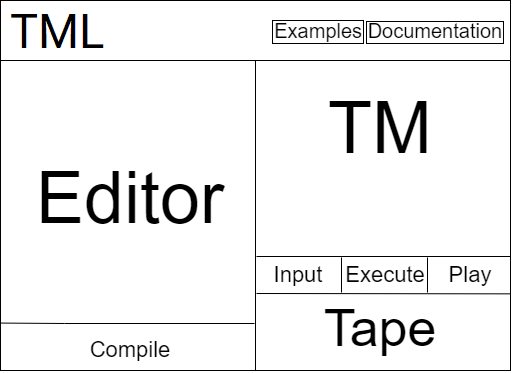
\includegraphics{images/Index webpage prototype.png}
    \caption{A prototype for the website homepage.}
    \label{fig:homepage_prototype}
\end{figure}

A prototype of the homepage was created to plan its layout. This is given in Figure \ref{fig:homepage_prototype}. The editor is placed on the left; the TM on the upper half of the right section; and the tape execution on bottom right. The toolbar features a button to go to the documentation, along with the ability to fill the editor with some example code. The editor can be compiled to a TM, and executed on a tape after the user types an input value. The execute button performs one step in execution, while the play button continually executes the program until it terminates. Note that this does not completely match the implementation.

\subsection{TM Conversion}
The website allows live conversion of a (valid) TML program into a TM. This includes constructing the FSM representation of a TM from the program. This is the main conversion since it is quite easy to follow the diagram during execution. To help the user do so, the current state/transition is also highlighted in the FSM.

\begin{table}[htb]
    \centering
    \begin{tabular}{c|ccc}
        & $0$ & $1$ & $\#$ \\
        \hline
        $q_0$ & $(R, 0, q_0)$ & $(R, 1, q_0)$ & $(L, \#, q_1)$ \\
        $q_1$ & $(L, 0, q_A)$ & $(L, 1, q_R)$ & $(L, 1, q_R)$ 
    \end{tabular}
    \caption{A transition table.}
    \label{tbl:table_isDiv2}
\end{table}

The website also allows the user to convert a TML program into a formal definition of a TM program. The result defines all the states and then presents a transition table, such as the one in Table \ref{tbl:table_isDiv2}. In this example, the non-terminating states are $q_0$ and $q_1$, and the alphabet $\Sigma = \{0, 1\}$. Moreover, the transition table says that $\delta(q_0, 0) = (R, 0, q_0)$, meaning that, during execution:
\begin{itemize}
    \item the tapehead pointer moves to the \emph{right};
    \item the tapehead value stays $\emph{0}$; and 
    \item the current state remains $\emph{q}_\emph{0}$
\end{itemize}

\subsection{Tape Execution}
The user can input a valid string in the alphabet and execute the TML program on a tape. The tape panel feature 15 visible tape entries (spots for an input value). The tape panel animates the execution process in the tape entries, which involves:
\begin{itemize}
    \item changing the tapehead value; and
    \item moving the tape to the left or the right.
\end{itemize}
Note that a \textit{move} command moves the \textit{pointer}, not the tape. Hence, the command \texttt{move left} moves the \textit{tape} to the right; the tapehead position remains constant.

\begin{figure}[htb]
    \centering
    \begin{subfigure}{0.3\textwidth}
        \centering
        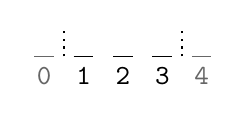
\begin{tikzpicture}
            \foreach \x in {0, 4} {
                \draw[opacity=0.6] (\x*0.5, 0) -- (\x*0.5+0.25, 0);
                \node[opacity=0.6] at (\x*0.5+0.125, -0.25) {\texttt{\x}};
            }
            \foreach \x in {1, 2, 3} {
                \draw (\x*0.5, 0) -- (\x*0.5+0.25, 0);
                \node at (\x*0.5+0.125, -0.25) {\texttt{\x}};
            }

            \draw[thick, dotted] (0.375, 0) -- (0.375, 0.35);
            \draw[thick, dotted] (1.875, 0) -- (1.875, 0.35);
        \end{tikzpicture}
        \caption{}
    \end{subfigure}
    \hfill
    \begin{subfigure}{0.3\textwidth}
        \centering
        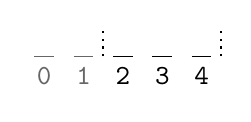
\begin{tikzpicture}
            \foreach \x in {0, 1} {
                \draw[opacity=0.6] (\x*0.5, 0) -- (\x*0.5+0.25, 0);
                \node[opacity=0.6] at (\x*0.5+0.125, -0.25) {\texttt{\x}};
            }
            \foreach \x in {2, 3, 4} {
                \draw (\x*0.5, 0) -- (\x*0.5+0.25, 0);
                \node at (\x*0.5+0.125, -0.25) {\texttt{\x}};
            }

            \draw[thick, dotted] (0.875, 0) -- (0.875, 0.35);
            \draw[thick, dotted] (2.375, 0) -- (2.375, 0.35);
        \end{tikzpicture}
        \caption{}
    \end{subfigure}
    \hfill
    \begin{subfigure}{0.3\textwidth}
        \centering
        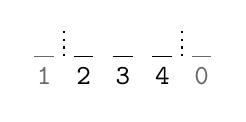
\begin{tikzpicture}
            \foreach \x[evaluate={int(mod(\x, 5))} as \y] in {5, 1} {
                \draw[opacity=0.6] (\x*0.5, 0) -- (\x*0.5+0.25, 0);
                \node[opacity=0.6] at (\x*0.5+0.125, -0.25) {\texttt{\y}};
            }

            \foreach \x in {2, 3, 4} {
                \draw (\x*0.5, 0) -- (\x*0.5+0.25, 0);
                \node at (\x*0.5+0.125, -0.25) {\texttt{\x}};
            }

            \draw[thick, dotted] (0.875, 0) -- (0.875, 0.35);
            \draw[thick, dotted] (2.375, 0) -- (2.375, 0.35);
        \end{tikzpicture}
        \caption{}
    \end{subfigure}
    \caption{The transition process for tape entries.}
    \label{fig:tape_movement}
\end{figure}

For the tape movement animation to look smooth, there are always 2 tape entries to either side of the tape. That way, if the tape gets moved to left or right, there will be a tape entry to show. This is illustrated in Figure \ref{fig:tape_movement} (a)- the tape entries 0 and 4 are out of frame and therefore invisible. 

When the tape moves, there will be 2 tape entries on one side. For instance, if the tape moves to the left in Figure \ref{fig:tape_movement} (a), then we get Figure \ref{fig:tape_movement} (b). After the transition has completed, we instantly move the most extreme tape entry to the other side. In the example, we move tape entry 0 to the right, leading to the tape state given in Figure \ref{fig:tape_movement} (c). At this point, we also change the tape value of entry 0 so that it matches tape value at index 5.
